\documentclass[]{scrreprt}
\usepackage{amsmath,amsfonts,graphicx}
\usepackage{multirow}
\usepackage{pslatex}
\usepackage{tabularx}
\usepackage{comment}
\usepackage{xspace}
\usepackage{array}

\usepackage{hyperref}

\usepackage{caption}
\DeclareCaptionFont{white}{\color{white}}
\DeclareCaptionFormat{listing}{\colorbox{gray}{\parbox{\textwidth}{#1#2#3}}}

\graphicspath{
{figures/}
}

\newcommand{\uo}{\mbox{UO\textsubscript{2}}\xspace}

\setcounter{secnumdepth}{3}


\begin{document}


\title{Fracture Flow}
\author{Andy Wilkins \\
CSIRO}
\maketitle

\tableofcontents

%%%
\chapter{Introduction}
%%%

Flow through a microscopic fracture coupled with flow through a
macroscopic medium is interesting in many geological settings, such as
study of coal-seam gas reservoirs.  Superficially quite dissimilar,
but almost identical as far as MOOSE is concerned is the coupling of
surface-water flows with groundwater flows.  Both these applications involve
coupling physics on an essentially 2D surface with physics in a 3D
medium.

In this document I demonstrate that this type of coupling is
astonishingly simple in MOOSE.  In fact {\em no extra C++ code needs
  be written} usually!  All that needs be done is to write and
benchmark the individual physics {\em separately} --- eg groundwater
physics and surface water physics --- and then couple them together
using a specially designed mesh.  All the work then reduces to the
mesh creation: a preprocessing stage!

This mesh needs two types of blocks of elements: blocks containing 3D
elements; and blocks containing the 2D surface elements.  The 2D
elements must be faces of a 3D element.   In cubit or trelis this step
is accomplished by the simple {\tt imprint all} and {\tt merge all}
operations.  This is necessary so that the 2D physics ``feels'' the 3D
physics, and viceversa, otherwise the two physics will run separately
without any coupling.  The idea is shown in Figure~\ref{bdy_bulk.fig}.

\begin{figure}[htb]
\centering
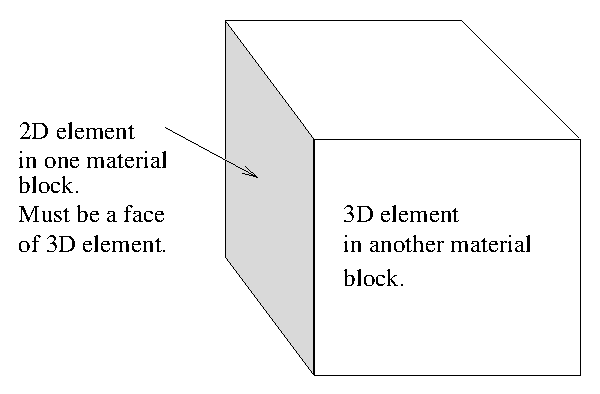
\includegraphics[width=6cm]{bdy_bulk.eps}
\caption{Type of mesh needed when coupling 2D surface physics with 3D
  bulk physics.}
\label{bdy_bulk.fig}
\end{figure}


\chapter{Solute Diffusion into a Porous Matrix from a Single Fracture}

Here I work through in detail a benchmark test described in Section
14.5 of the FEFLOW book\footnote{H-J G Diersch ``FEFLOW Finite Element
  Modeling of Flow, Mass and Heat Transport in Porous and Fractured
  Media'' Springer 2014}.  This test is based on analytic results from
Tang, Frind and Sudicky\footnote{DH Tang, EO FRind and EA Sudicky
  ``Contaminant transport in fractured porous media: Analytical
  solution for a single fracture'' Water Resources Research 17 (1981)
  555-564}.  There is also a useful finite element study using a
macroscropic-sized fracture in Grisak and Pickens\footnote{GE Grisak
  and JF Picken ``Solute transport through fractured media 1.  The
  effect of matrix diffusion'' Water Resources Research 16 (1980)
  719--730} in which the governing equations are carefully explained
and an analytical solution presented due to Carslaw and Jaeger which
is very similar to the ones found below.

The analytical solutions include the effect of diffusivity within the
fracture, as well as radioactive decay of the solute, but, following
FEFLOW, I do not consider those effects since I am wanting to
concentrate on the fracture-bulk coupling.  Hence the governing
equation for flow within the fracture and flow within the bulk is the
advection-diffusion equation:
\begin{equation}
\frac{\partial}{\partial t} \phi C - \nabla_{i}\left(\phi D_{ij}\nabla_{j}C\right)
+ \nabla_{i}\left(v_{i}C\right) = 0 \ .
\label{eqn.solute.de}
\end{equation}
In this equation:
\begin{itemize}
\item $t$ is time with dimensions [T], and $x_{i}$ with dimensions
  [L] are the three spatial dimensions
\item $C$ is the mass of solute per unit volume of solvent, with
  dimensions [M.L$^{-3}$], where M represents mass.
\item $\phi$ is the porosity.  This means $\phi C$ is the mass of
  solute per unit volume of the ``rock'' [M.L$^{-3}$].  Below $\phi$ will
  be unity within the fracture, since it is assumed to be fully filled
  with solvent, but less than unity in the bulk.
\item $D_{ij}$ is the anisotropic diffusivity tensor
  [L$^{2}$.T$^{-1}$], which is different in the fracture and in the bulk.  The analytical
  results are only valid for certain $D_{ij}$ as described below
\item $v_{i}$ is the solvent velocity, for instance provided through
  Darcy flow [L.T$^{-1}$].  The analytical results are only valid for certain
  $v_{i}$.
\end{itemize}
At an interface, such as a fracture wall, both
\begin{equation}
C \ \ \ \mbox{and}\ \ \ n_{i}(v_{i}C - \phi D_{ij}\nabla_{j}C) \ ,
\end{equation}
must be continuous.  The former is continuity of the concentration,
while the latter is continuity of the flux.


\section{Physics of a microscopic fracture}

Now consider a medium containing a single fracture, as depicted in
Figure~\ref{single.fig}.  The fracture sits in the region
$-a\leq x \leq a$.


\begin{figure}[htb]
\centering
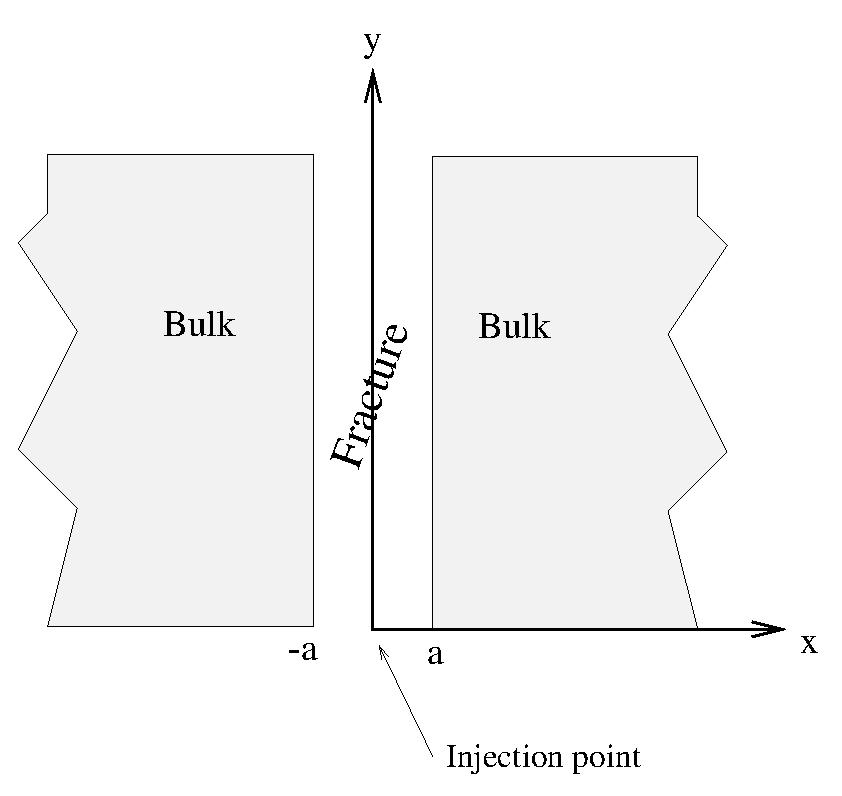
\includegraphics[width=7cm]{single.eps}
\caption{A single fracture sits in the region $-a\leq x \leq a$.  As
  described in the text, solute will be injected at $y=0$.}
\label{single.fig}
\end{figure}

In Grisak and Pickens both the fracture and the
bulk are discretised with 3D finite elements and
Eqn~(\ref{eqn.solute.de}) is solved with $\phi$, $D$ and $v$ being
different in the fracture and the bulk.  Here I want to take a
different approach, which is identical to FEFLOW as Tang, Frind and
Sudicky.  Assume
\begin{itemize}
\item $v_{x} = 0$ in the fracture;
\item $a^{2}/D_{xx}$ is tiny compared with any other timescale in the
  problem.
\end{itemize}
Then the solute concentration in the fracture will obey
\begin{equation}
\frac{\partial C}{\partial x} \approx 0 \ .
\end{equation}
This is the standard ``small aperture'' approximation.  To avoid
having to mesh the fracture\footnote{I am going to
  consider just the region $x>0$ in the MOOSE simulation.  If I were
  considering the full 3D domain, $-\infty < x < \infty$, then all the
  solute mass between $-a\leq x \leq a$ would be placed on a surface
  at $x=0$, and then the bulk translated by $a$ to create a sandwich.
  This means that there would be a factor of $2a$ instead of $a$ in
  Eqn~(\ref{eqn.solute.surface.de})} with 3D elements, {\em all the solute mass
between $0\leq x \leq a$ is placed on the surface at $x=a$}.  The DE
governing solute movement on this surface is therefore
\begin{equation}
\frac{\partial}{\partial t} \phi aC - \nabla_{i}\left(\phi D_{ij}\nabla_{j}aC\right)
+ \nabla_{i}\left(v_{i}aC\right) = 0 \ .
\label{eqn.solute.surface.de}
\end{equation}
Here $\phi$, $D$ and $v$ are parameters relevant for the fracture.
Of course one may trivially divide by\footnote{or $2a$ in the case of
  the previous footnote} $a$ and the same solution within the fracture
will be obtained, however Eqn~(\ref{eqn.solute.surface.de}) will
correctly count mass at a finite-element node, so may be used
straightforwardly in MOOSE when coupled with Eqn~(\ref{eqn.solute.de})
in the bulk.



\section{The analytical solution}

Tang, Frind and Sudicky derived the analytical solution under the
following assumptions.
\begin{itemize}
\item In the fracture $v_{x} = 0$, and $a^{2}/D_{xx}$ is
  inconsequential compared with any other timescale in the problem, so
  the fracture may be treated as described above.
\item The concentration is initially zero everywhere, and at time
  $t\geq 0$ the concentration of solute is fixed at the fracture entry:
\begin{equation}
C(x=a, y=0, t) = 1 \ .
\end{equation}
\item The boundary at $y=0$ is impermeable, and the domain is
  semi-infinite as suggested in Figure~\ref{single.fig}.
\item In the fracture $v_{y}$ is constant.  Also I (and FEFLOW) assume
  $D_{yy}=0$ in the fracture in order to simplify the formulae below.
  Hence solute simply advects up the fracture with a constant
  velocity.
\item In the bulk $v=0$, and also all components of $D$ are zero
  except $D_{xx}\neq 0$.
\end{itemize}
These assumptions mean that solute will advect in the $y$ direction
within the fracture.  It will leak to the bulk in the $x$ direction,
but will not diffuse in the $x$ direction within the bulk.  This is
depicted in Figure~\ref{single_flow.fig}

\begin{figure}[htb]
\centering
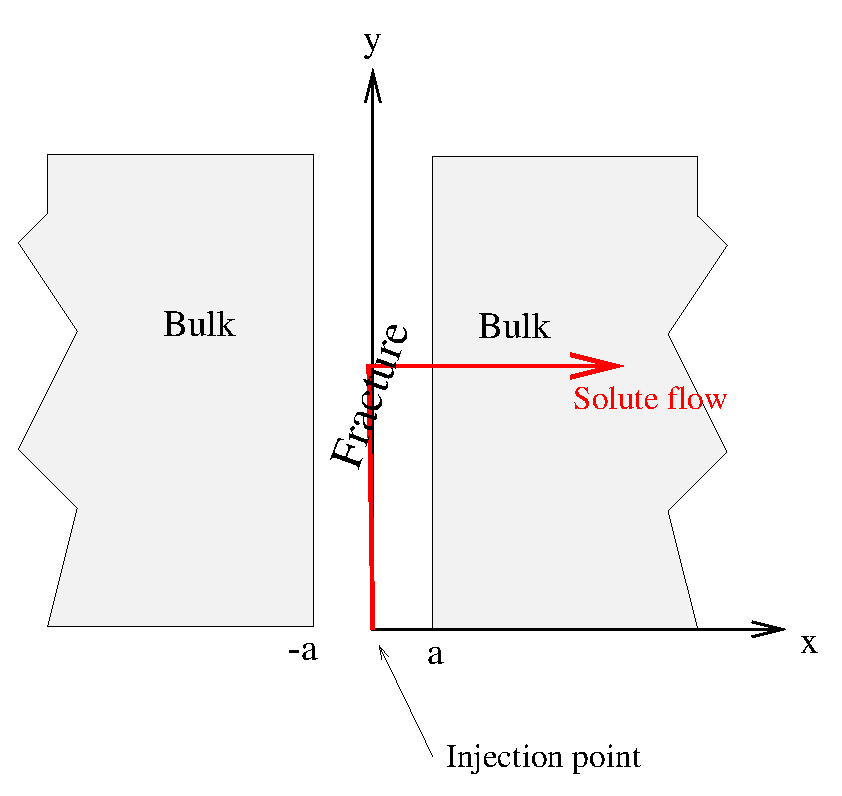
\includegraphics[width=6cm]{single_flow.eps}
\caption{Showing the solute flow direction is vertical within the
  fracture and horizontal within the bulk.}
\label{single_flow.fig}
\end{figure}

Define
\begin{equation}
\tau = t - \frac{y\phi^{\mathrm{frac}}}{v}\ ,
\end{equation}
which is positive for points in the fracture behind the advecting
front, and negative for those that haven't been touched by solute
yet.  Then
the analytic solution is
\begin{eqnarray}
C & = & \left\{
\begin{array}{ll}
\mbox{erfc}\left[
\frac{1}{2\sqrt{\tau}}
\left( \phi^{\mathrm{bulk}}\sqrt{D_{xx}^{\mathrm{bulk}}}
\frac{y}{av_{y}^{\mathrm{frac}}}
+ \frac{x-a}{\sqrt{D_{xx}^{\mathrm{bulk}}}} \right) \right]
& \mbox{for}\ \ \tau > 0 \\
0 & \mbox{for}\ \ \tau \leq 0 \\
\end{array}
\right.
\end{eqnarray}
This formula is correct, but note that there is a typo in both Tang,
Frind and Sudicky, and the FEFLOW manual which means the solution for
$x=a$ (at the fracture surface) is wrong unless the porosity of the
fracture is unity, which is fortunately the case studied in the FEFLOW
benchmark.  Here erfc is the complimentary error function.


\section{Comparison with MOOSE}

In a similar way to FEFLOW, the following simulation parameters are
used in MOOSE \\
\begin{center}
\begin{tabular}{ll}
\hline
{\em Domain} \\
Mesh width ($x$) & 1\,m \\
Mesh height ($y$) & 1\,m \\
Number of quad elements & $25\times 50$ (this is $x\times y$) \\
\hline
{\em Fracture} \\
Porosity, $\phi^{\mathrm{frac}}$ & 1 \\
Half-aperture, $a$, & 0.1\,m \\
Velocity, $v_{y}^{\mathrm{frac}}$ & 0.8\,m.s$^{-1}$ \\
\hline
{\em Bulk} \\
Porosity, $\phi^{\mathrm{bulk}}$ & 0.2 \\
Diffusivity, $D_{xx}^{\mathrm{bulk}}$ & 0.01\,m$^{2}$.s$^{-1}$ \\
\hline
\end{tabular}
\end{center}
The simulation is run for 1\,s.

Figure~\ref{single_contoured.fig} depicts the solute concentration at
$t=1$\,s, and comparisons with the analytical results are shown in
Figure~\ref{single_results.fig}.  The
timestep has a large influence on the result.  The results depicted
below use $\Delta t = 0.002$\,s, and by decreasing the timestep the
results agree more closely with the analytical results.  In the test
suite this simulation is marked ``heavy''.  There is a non-heavy test
that uses $\Delta t = 0.1$\,s that is run automatically every time
MOOSE is updated.  Better agreement would probably be obtained by
lumping the mass and using upwinding, however, such features concern
the individual physics (2D fracture flow, or 3D bulk flow) and have
nothing to do with the coupling that is being tested here.


\begin{figure}[htb]
\centering
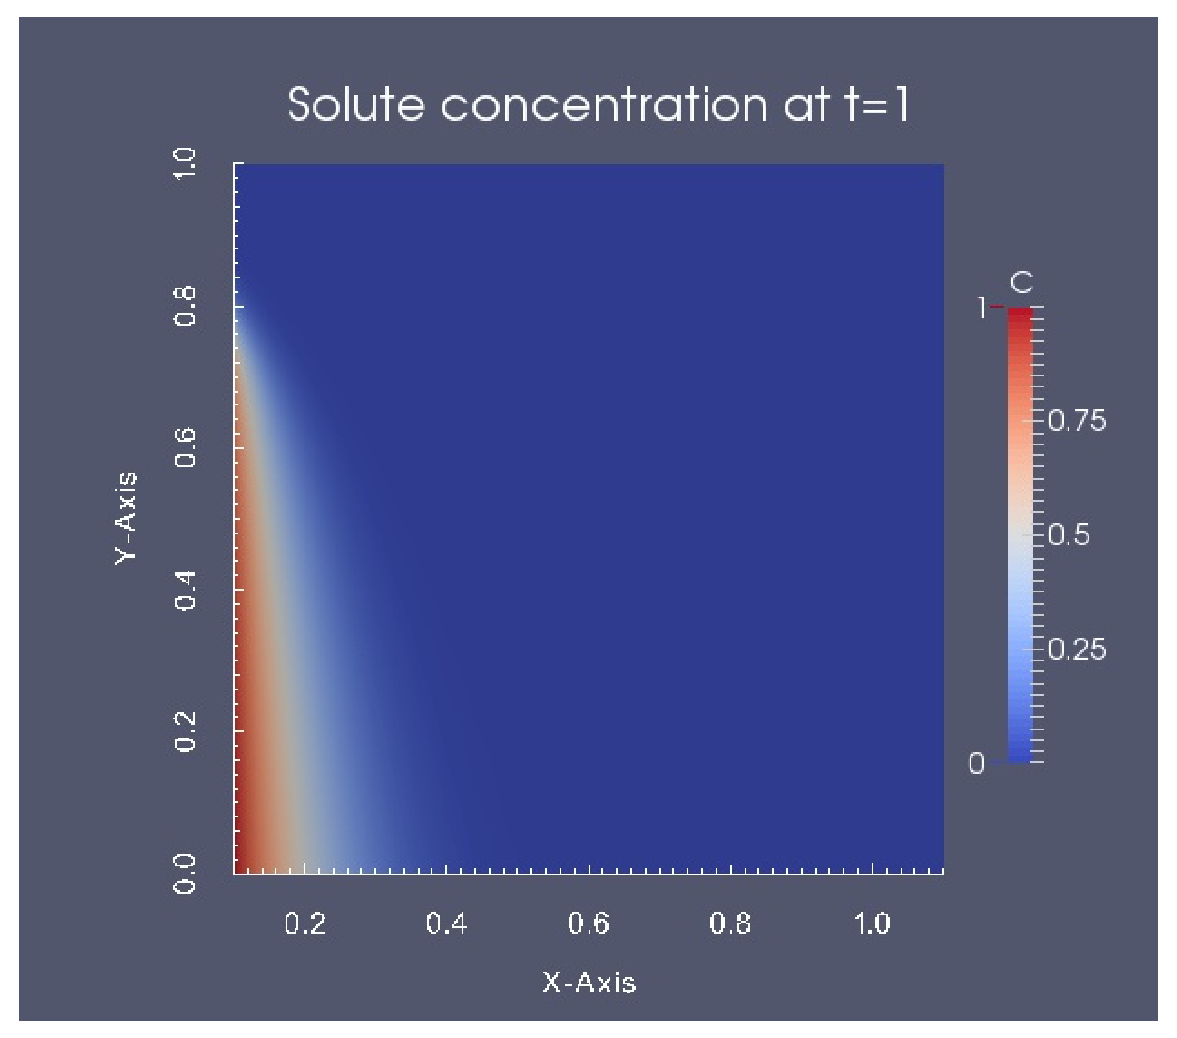
\includegraphics[width=8cm]{single_contoured.eps}
\caption{Contour of the solute concentration at $t=1$\,s}.
\label{single_contoured.fig}
\end{figure}

\begin{figure}[p]
\centering
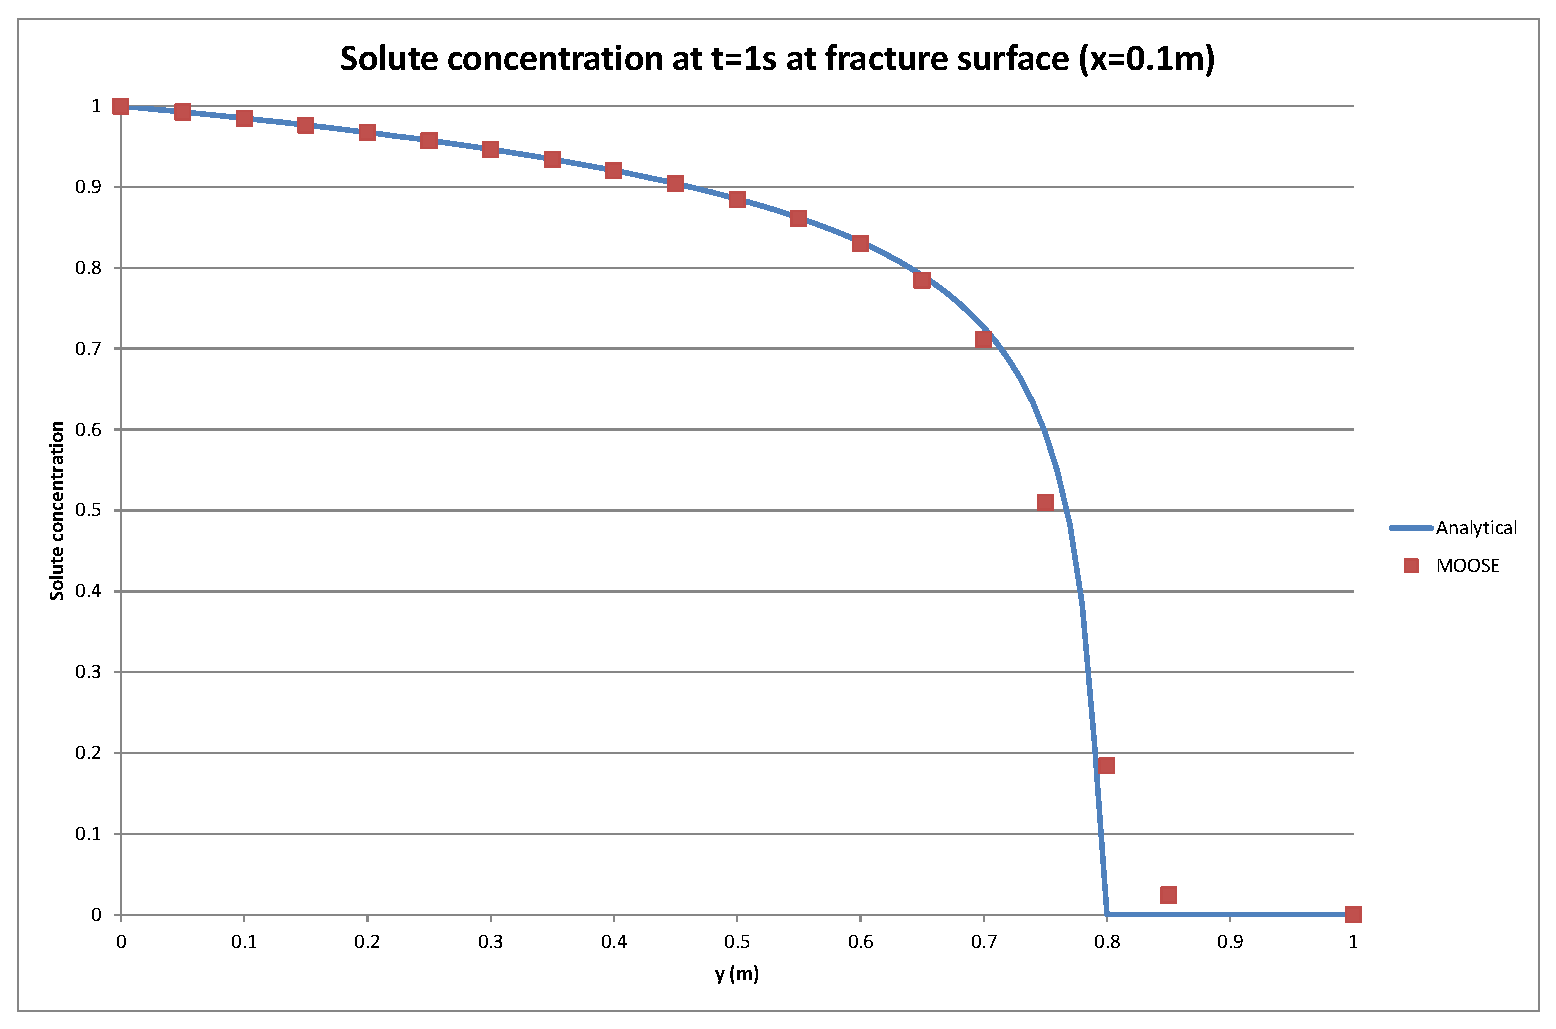
\includegraphics[width=8cm]{single_0.1.eps} \\
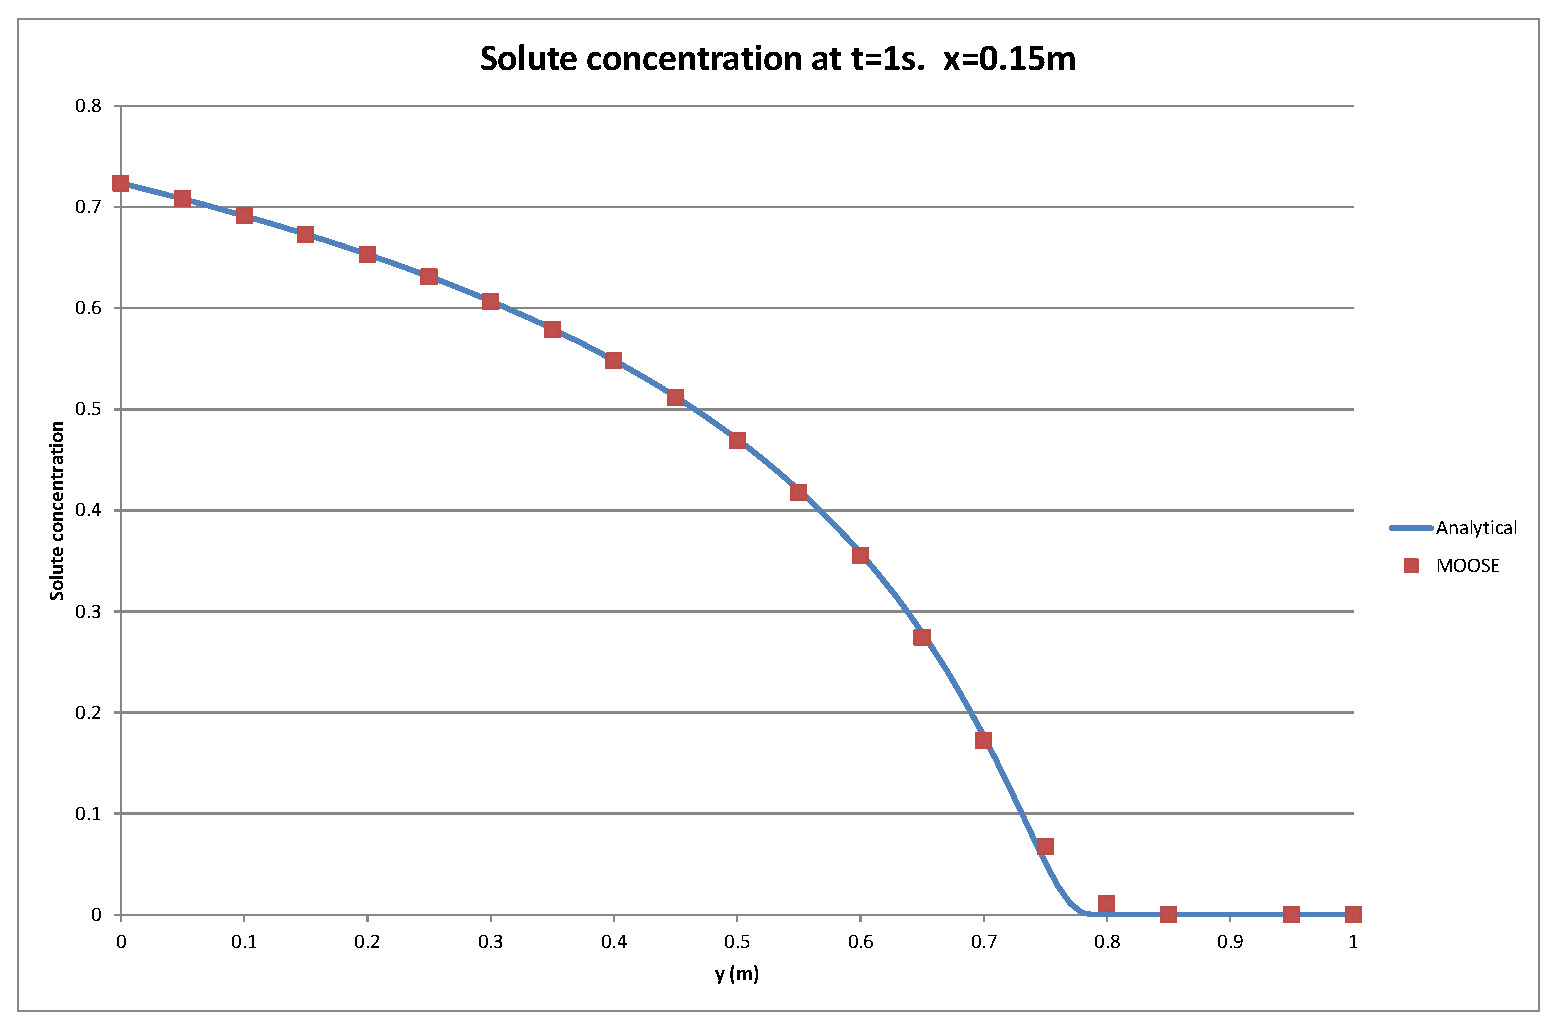
\includegraphics[width=8cm]{single_0.15.eps} \\
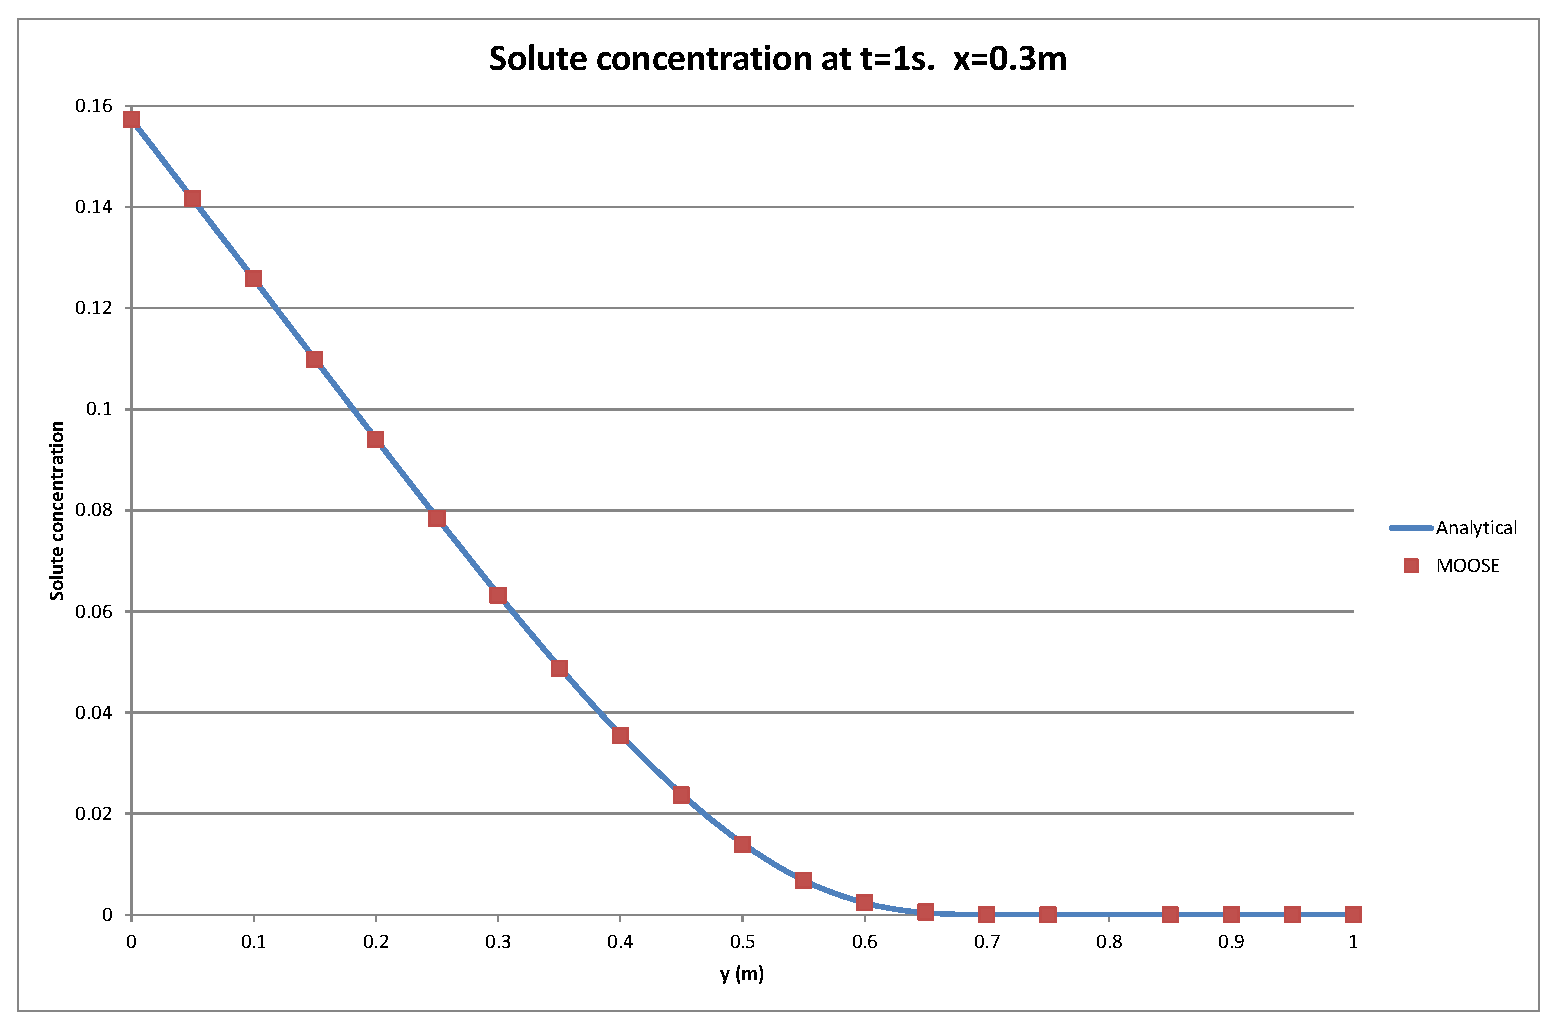
\includegraphics[width=8cm]{single_0.3.eps}
\caption{Comparison of MOOSE simulation results with the analytical
  results.  The agreement around the sharp front is improved by using
  finer spatial resolution or smaller $\Delta t$.}
\label{single_results.fig}
\end{figure}


\end{document}
